% !TeX program = xelatex
\documentclass[a4paper,10pt]{article}

% ============================================================================
% សន្លឹកកិច្ចការសិស្សបំពេញចន្លោះ ស-ខ្មៅ និងប្លង់ក្ដារខៀន/ចម្លើយគ្រូ (គ្មាន LCD / គ្មានកន្ត្រៃ)
% មេរៀនទី២ (៣.)៖ ចំនួនបឋម និងចំនួនមិនបឋម — ត្រូវគ្នា ១០០% នឹង LS_Plan_DIV23.tex
% ============================================================================
\usepackage[a4paper, left=1.0cm, right=1.0cm, top=0.75cm, bottom=1.00cm, footskip=0.52cm]{geometry}
\usepackage{amsmath}
\usepackage{unicode-math}
\usepackage{fontspec}
\usepackage{array, colortbl}
\usepackage[table]{xcolor}
\usepackage{enumitem}
\usepackage{pifont}
\usepackage{fancyhdr}
\usepackage{lastpage}
\usepackage{tikz}
\usepackage[most]{tcolorbox}
\usetikzlibrary{calc, arrows.meta, decorations.pathreplacing, positioning, babel}

\makeatletter
\let\@expl@@@mark@update@singlecol@structures@@\relax
\makeatother

\providecommand{\NGSFindFonts}{%
  \IfFileExists{C:/Windows/Fonts/cambria.ttc}{%
    \def\NGSSysPath{C:/Windows/Fonts/}%
    \def\NGSUserPath{C:/Users/KIT/AppData/Local/Microsoft/Windows/Fonts/}%
  }{%
    \IfFileExists{./fonts/KhmerOSsiemreap.ttf}{\def\NGSSysPath{./fonts/}\def\NGSUserPath{./fonts/}}{%
    \IfFileExists{../fonts/KhmerOSsiemreap.ttf}{\def\NGSSysPath{../fonts/}\def\NGSUserPath{../fonts/}}{%
    \IfFileExists{../../fonts/KhmerOSsiemreap.ttf}{\def\NGSSysPath{../../fonts/}\def\NGSUserPath{../../fonts/}}{%
    \IfFileExists{../../../fonts/KhmerOSsiemreap.ttf}{\def\NGSSysPath{../../../fonts/}\def\NGSUserPath{../../../fonts/}}{%
    \IfFileExists{../../../../fonts/KhmerOSsiemreap.ttf}{\def\NGSSysPath{../../../../fonts/}\def\NGSUserPath{../../../../fonts/}}{%
    \IfFileExists{../../../../../fonts/KhmerOSsiemreap.ttf}{\def\NGSSysPath{../../../../../fonts/}\def\NGSUserPath{../../../../../fonts/}}{%
    \IfFileExists{../../../../../../fonts/KhmerOSsiemreap.ttf}{\def\NGSSysPath{../../../../../../fonts/}\def\NGSUserPath{../../../../../../fonts/}}{%
      \def\NGSSysPath{../../../../../../../fonts/}\def\NGSUserPath{../../../../../../../fonts/}%
    }}}}}}}%
  }%
}
\NGSFindFonts

\setmathfont[Path={\NGSSysPath}, FontIndex=1, Scale=1.02]{cambria.ttc}
\defaultfontfeatures{Ligatures=TeX}

\setmainfont[
  Path={\NGSUserPath}, Extension=.ttf, Script=Khmer,
  BoldFont={KhmerOSsiemreap}, BoldFeatures={FakeBold=1.8},
  ItalicFont={KhmerOSsiemreap}, ItalicFeatures={FakeSlant=0.25},
  BoldItalicFont={KhmerOSsiemreap}, BoldItalicFeatures={FakeBold=1.8, FakeSlant=0.25}
]{KhmerOSsiemreap}

\newfontfamily\muol[Path={\NGSUserPath}, Extension=.ttf, Script=Khmer]{KhmerOSmuollight}
\newfontfamily\TimesEn[Path={\NGSSysPath}, Extension=.ttf, BoldFont={timesbd}, ItalicFont={timesi}, BoldItalicFont={timesbi}]{times}
\newfontfamily\CalibriFont[Path={\NGSSysPath}, Extension=.ttf]{calibri}

\XeTeXlinebreaklocale "km"
\XeTeXlinebreakskip = 0pt plus 1pt minus 0.1pt

\definecolor{panelgray}{gray}{0.94}
\definecolor{headgray}{gray}{0.85}

\pagestyle{fancy}
\fancyhf{}
\renewcommand{\headrulewidth}{0pt}
\fancyfoot[L]{\fontsize{7.4pt}{9.5pt}\selectfont អនុវិទ្យាល័យព្រះក្រសាំង \en{|} គ្រូ៖ ហុក ប៊ុនថែន \en{|} មេរៀនទី២ (៣.) ចំនួនបឋម និងចំនួនមិនបឋម \en{|} ថ្ងៃសៅរ៍ ទី១៤ ខែវិច្ឆិកា ឆ្នាំ២០២៦}
\fancyfoot[R]{\fontsize{7.8pt}{10pt}\selectfont ទំព័រ \en{\thepage\ / \pageref{LastPage}}}

\setlength{\parindent}{0pt}
\setlength{\parskip}{0pt}
\setlength{\tabcolsep}{4pt}
\newcolumntype{L}[1]{>{\raggedright\arraybackslash}p{#1}}
\newcolumntype{C}[1]{>{\centering\arraybackslash}p{#1}}

\newcommand{\en}[1]{{\TimesEn #1}}
\newcommand{\enbf}[1]{{\TimesEn\bfseries #1}}
\newcommand{\unit}[1]{\,\text{\en{#1}}}
\newcommand{\cnum}[1]{\mbox{\fontsize{10pt}{12pt}\selectfont\ding{\numexpr181+#1\relax}}}
\newcommand{\chkbox}{\tikz[baseline=-0.15ex]\draw[black, line width=0.85pt, fill=white] (0,0) rectangle (0.24cm,0.24cm);}
\newcommand{\ansbox}[1][1.75cm]{\,\tikz[baseline=-0.65ex]\draw[black, line width=0.65pt, fill=white] (0,0) rectangle (#1, 0.42cm);\,}
\newcommand{\dotline}[1][2.2cm]{\makebox[#1]{\dotfill}}

\newcommand{\pagebanner}[2]{%
  \begin{tcolorbox}[
    enhanced, sharp corners, colback=headgray, colframe=black,
    boxrule=1.05pt, boxsep=1pt, top=2.5pt, bottom=2.5pt, left=6pt, right=6pt,
    after skip=3.5pt
  ]
    {\muol\fontsize{9.0pt}{13.2pt}\selectfont #1}\hfill{\fontsize{8.0pt}{11.2pt}\selectfont\textbf{#2}}
  \end{tcolorbox}%
}

\newcommand{\secstrip}[2]{%
  \vspace{3pt}%
  \begin{tcolorbox}[
    enhanced, sharp corners, colback=panelgray, colframe=black,
    boxrule=0.8pt, boxsep=0.8pt, top=2pt, bottom=2pt, left=5pt, right=5pt,
    after skip=3pt
  ]
    {\muol\fontsize{8.5pt}{12.2pt}\selectfont #1}\hfill{\fontsize{7.8pt}{10.8pt}\selectfont\textit{#2}}
  \end{tcolorbox}%
}

\begin{document}
\fontsize{9.5pt}{14.5pt}\selectfont

% ============================================================================
% ទំព័រទី ១៖ សន្លឹកកិច្ចការសិស្ស (ផ្នែកមុខ៖ E1 -> E2 -> E3)
% ============================================================================
\pagebanner{សន្លឹកកិច្ចការសិស្ស \enbf{(}៣\enbf{.} ចំនួនបឋម និងចំនួនមិនបឋម\enbf{)} \enbf{--} ផ្នែកមុខ}{ថ្នាក់ទី៧ \en{|} សៀវភៅគោល ទំ.១៩}

\begin{tcolorbox}[
  enhanced, sharp corners, colback=white, colframe=black,
  boxrule=0.8pt, boxsep=1.5pt, top=3.5pt, bottom=3.5pt, left=5pt, right=5pt,
  after skip=4pt
]
  \fontsize{9.0pt}{13.0pt}\selectfont
  \textbf{ឈ្មោះសិស្ស៖} \dotline[4.3cm] \quad
  \textbf{សមាជិកក្រុម៖} \dotline[4.3cm] \quad
  \textbf{ថ្នាក់ទី៖} ៧\dotline[0.9cm] \quad
  \textbf{ក្រុមទី៖} \dotline[1.0cm]
\end{tcolorbox}

% --- E1 Engage ---
\secstrip{ផ្នែកទី ១ \enbf{(E1 - Engage)} ៖ បេសកកម្មអន្ទាក់គូ/សេស និងលេខ \enbf{1, 2, 9}}{រយៈពេល ៣ នាទី (គូស \ding{51} ក្នុង \chkbox)}

\begin{tcolorbox}[
  enhanced, sharp corners, colback=white, colframe=black,
  boxrule=0.8pt, boxsep=2pt, top=4pt, bottom=4pt, left=6pt, right=6pt
]
  សិស្សពីរនាក់ជជែកគ្នាអំពីលេខ $1,\ 2$ និង $9$ ៖\\[2.5pt]
  $\bullet$ \chkbox\ \textbf{សិស្ស ក៖} «$1$ និង $9$ ជាចំនួនបឋមព្រោះជាចំនួនសេស រីឯ $2$ មិនមែនចំនួនបឋមទេព្រោះជាចំនួនគូ!»\\[2pt]
  $\bullet$ \chkbox\ \textbf{សិស្ស ខ៖} «មិនមែនមើលគូឬសេសទេ គឺត្រូវរាប់\textbf{ចំនួនតួចែក}! $2$ មានតួចែកតែពីរគត់ ($1, 2$) រីឯ $9$ មានតួចែកបី ($1, 3, 9$)!»
\end{tcolorbox}

\vfill

% --- E2 Explore ---
\secstrip{ផ្នែកទី ២ \enbf{(E2 - Explore)} ៖ ការរាប់ចំនួនតួចែក និងកញ្ច្រែងអេរ៉ាតូស្ដែន (ទំ.១៩)}{រយៈពេល ១១ នាទី}

\textbf{សកម្មភាព ១ (\en{E2-A} — ៥ នាទី)៖ រាយតួចែក និងធ្វើចំណាត់ថ្នាក់ចំនួនគត់តាមចំនួនតួចែក (សៀវភៅគោល ទំ.១៩)}

{\renewcommand{\arraystretch}{1.35}
\begin{tabular}{|C{1.4cm}|L{5.6cm}|C{3.2cm}|L{7.2cm}|}
\hline
\cellcolor{headgray}\textbf{ចំនួន} &
\multicolumn{1}{c|}{\cellcolor{headgray}\textbf{តួចែកទាំងអស់}} &
\cellcolor{headgray}\textbf{ចំនួនតួចែក} &
\multicolumn{1}{c|}{\cellcolor{headgray}\textbf{ប្រភេទចំនួន (បឋម / មិនបឋម / ពិសេស)}} \\
\hline
$\mathbf{5}$ & $1,\ 5$ & $2$ តួចែកគត់ & \textbf{ចំនួនបឋម} \\ \hline
$\mathbf{14}$ & $1,\ 2,$ \dotline[0.8cm], \dotline[0.8cm] & \dotline[1.0cm] តួចែក & \dotline[4.5cm] \\ \hline
$\mathbf{15}$ & $1,$ \dotline[0.8cm], \dotline[0.8cm], $15$ & \dotline[1.0cm] តួចែក & \dotline[4.5cm] \\ \hline
$\mathbf{23}$ & $1,$ \dotline[0.9cm] & \dotline[1.0cm] តួចែក & \dotline[4.5cm] \\ \hline
$\mathbf{2}$ & $1,$ \dotline[0.8cm] & \dotline[1.0cm] តួចែក & \dotline[4.5cm] \\ \hline
$\mathbf{1}$ & $1$ & \dotline[1.0cm] តួចែកគត់ & \textbf{មិនមែនបឋម និងមិនមែនមិនបឋម} \\ \hline
\end{tabular}}

\vspace{4pt}
\textbf{សកម្មភាព ២ (\en{E2-B} — ៦ នាទី)៖ អនុវត្តកញ្ច្រែងអេរ៉ាតូស្ដែនលើចំនួន $1$ ដល់ $20$}

\begin{tcolorbox}[
  enhanced, sharp corners, colback=white, colframe=black,
  boxrule=0.8pt, boxsep=2.5pt, top=4pt, bottom=4pt, left=6pt, right=6pt
]
  \textbf{សេចក្ដីណែនាំ៖} (១) គូសខ្វែង $\times$ លើលេខ $1$; \quad (២) គូសរង្វង់ $\bigcirc$ លេខ $2$ រួចឆូតចោលពហុគុណនៃ $2$ ($4,6,\dots,20$); \quad (៣) គូសរង្វង់ $\bigcirc$ លេខ $3$ រួចឆូតពហុគុណនៃ $3$ ($9, 15$) ហើយគូសរង្វង់ចំនួនដែលនៅសល់ទាំងអស់៖\par\vspace{3.5pt}
  {\centering\renewcommand{\arraystretch}{1.35}
  \begin{tabular}{|*{10}{C{1.42cm}|}}
  \hline
  $1$ & $2$ & $3$ & $4$ & $5$ & $6$ & $7$ & $8$ & $9$ & $10$ \\ \hline
  $11$ & $12$ & $13$ & $14$ & $15$ & $16$ & $17$ & $18$ & $19$ & $20$ \\ \hline
  \end{tabular}\par}
\end{tcolorbox}

\vfill

% --- E3 Explain ---
\secstrip{ផ្នែកទី ៣ \enbf{(E3 - Explain)} ៖ និយមន័យទូទៅ និងធនាគារហេតុផល \enbf{B\&W}}{រយៈពេល ៦ នាទី}

\begin{tcolorbox}[
  enhanced, sharp corners, colback=white, colframe=black,
  boxrule=0.85pt, boxsep=2.5pt, top=4pt, bottom=4pt, left=6pt, right=6pt
]
  ១) \textbf{ចំនួនបឋម} គឺជាចំនួនគត់ធំជាង $1$ ដែលមានតួចែក \dotline[2.2cm] គឺ $1$ និង \dotline[1.8cm] ។\\[2.5pt]
  ២) \textbf{ចំនួនមិនបឋម} គឺជាចំនួនគត់ធំជាង $1$ ដែលមានតួចែក \dotline[2.8cm] ។\\[2.5pt]
  ៣) \textbf{សម្គាល់ (ទំ.១៩)៖} លេខ «\dotline[0.8cm]» មិនមែនជាចំនួនបឋម និងមិនមែនជាចំនួនមិនបឋមទេ រីឯលេខ «\dotline[0.8cm]» ជាចំនួនបឋមគូតែមួយគត់ ។\\[3.5pt]
  \tikz\draw[black, dashed, line width=0.5pt] (0,0) -- (18.4cm,0);\\[3pt]
  \fontsize{8.7pt}{12.8pt}\selectfont
  \textbf{ធនាគារហេតុផល (\en{Warrant Bank})៖} \quad
  \cnum{1} ចំនួនបឋម ($>1$, មានតួចែក $2$ គត់៖ $1$ និងខ្លួនឯង) \quad
  \cnum{2} ចំនួនមិនបឋម ($>1$, មានតួចែក $>2$)\\
  \cnum{3} ករណីពិសេស ($1$ មានតួចែកតែ $1$; $2$ ជាបឋមគូតែមួយគត់) \quad
  \cnum{4} កញ្ច្រែងអេរ៉ាតូស្ដែន $<50$ (ឆូត $1$ និងពហុគុណនៃ $2, 3, 5, 7$)
\end{tcolorbox}

% ============================================================================
% ទំព័រទី ២៖ សន្លឹកកិច្ចការសិស្ស (ផ្នែកខាងខ្នង៖ E4 -> E5 -> កិច្ចការផ្ទះ)
% ============================================================================
\clearpage
\pagebanner{សន្លឹកកិច្ចការសិស្ស \enbf{(}៣\enbf{.} ចំនួនបឋម និងចំនួនមិនបឋម\enbf{)} \enbf{--} ផ្នែកខាងខ្នង}{ថ្នាក់ទី៧ \en{|} សៀវភៅគោល ទំ.១៩ និង ទំ.២៤}

% --- E4 Elaborate ---
\secstrip{ផ្នែកទី ៤ \enbf{(E4 - Elaborate)} ៖ លំហាត់គំរូតាមសៀវភៅគោល ទំ.១៩}{រយៈពេល ១០ នាទី}

\begin{tcolorbox}[
  enhanced, sharp corners, colback=white, colframe=black,
  boxrule=0.8pt, boxsep=2.5pt, top=4pt, bottom=4pt, left=6pt, right=6pt
]
  $\bullet$ \textbf{ក.} រកចំនួនបឋមទាំងអស់ដែលនៅចន្លោះ $1$ និង $20$៖ \ansbox[8.8cm] (\cnum{1}, \cnum{3})\\[3.5pt]
  $\bullet$ \textbf{ខ.} រកចំនួនមិនបឋមដែលជា\textbf{ចំនួនគត់សេស}នៅចន្លោះ $1$ និង $30$៖ \ansbox[7.5cm] (\cnum{2})\\[3pt]
  \fontsize{8.8pt}{12.6pt}\selectfont
  \textbf{ឆ្លុះបញ្ចាំង (\en{EIA Looking-Back})៖} ពេលរែងរកចំនួនបឋមតូចជាង $50$ ហេតុអ្វីយើងឆូតត្រឹមពហុគុណនៃ $2, 3, 5, 7$ មិនបាច់ឆូតពហុគុណនៃ $11$ ទៀត? ព្រោះ $11\times 11 =$ \dotline[1.4cm] $> 50$!
\end{tcolorbox}

\vfill

% --- E5 Evaluate ---
\secstrip{ផ្នែកទី ៥ \enbf{(E5 - Evaluate)} ៖ ប្រតិបត្តិកញ្ច្រែងអេរ៉ាតូស្ដែន \enbf{1--50} (ទំ.១៩) និងសំណួរវិនិច្ឆ័យ}{រយៈពេល ១០ នាទី}

\begin{tcolorbox}[
  enhanced, sharp corners, colback=white, colframe=black,
  boxrule=0.8pt, boxsep=2.5pt, top=4pt, bottom=4pt, left=6pt, right=6pt
]
  \textbf{១) ប្រតិបត្តិជាក្រុមតូច ៣ នាក់ (សៀវភៅគោល ទំ.១៩)៖ រកចំនួនបឋមទាំងអស់ដែលតូចជាង $50$}\\[2.5pt]
  \fontsize{8.8pt}{12.5pt}\selectfont
  \textbf{ជំហានអនុវត្ត (\cnum{4})៖} គូសខ្វែង $\times$ លើ $1$ $\to$ គូសរង្វង់ $2, 3, 5, 7$ ហើយឆូតគ្រប់ពហុគុណរបស់វា (ប្រយ័ត្នលេខ $49 = 7\times 7$!) រួចគូសរង្វង់ចំនួននៅសល់៖\par\vspace{3.5pt}
  {\centering\renewcommand{\arraystretch}{1.28}
  \begin{tabular}{|*{10}{C{1.42cm}|}}
  \hline
  $1$ & $2$ & $3$ & $4$ & $5$ & $6$ & $7$ & $8$ & $9$ & $10$ \\ \hline
  $11$ & $12$ & $13$ & $14$ & $15$ & $16$ & $17$ & $18$ & $19$ & $20$ \\ \hline
  $21$ & $22$ & $23$ & $24$ & $25$ & $26$ & $27$ & $28$ & $29$ & $30$ \\ \hline
  $31$ & $32$ & $33$ & $34$ & $35$ & $36$ & $37$ & $38$ & $39$ & $40$ \\ \hline
  $41$ & $42$ & $43$ & $44$ & $45$ & $46$ & $47$ & $48$ & $49$ & $50$ \\ \hline
  \end{tabular}\par}
  \vspace{3.5pt}
  \fontsize{9.2pt}{13.5pt}\selectfont
  $\bullet$ ដូចនេះ ចំនួនបឋមតូចជាង $50$ មាន \dotline[0.9cm] ចំនួនគឺ៖ \dotline[11.2cm]\\[2.5pt]
  \hspace*{0.3cm}\dotline[17.6cm]\\[3pt]
  \textbf{២) បិទបេសកកម្ម \en{E1}៖} សិស្ស \dotline[1.0cm] ត្រឹមត្រូវ! $2$ ជា\dotline[2.4cm], $9$ ជា\dotline[2.4cm] រីឯ $1$ \dotline[3.6cm] ។
\end{tcolorbox}

\vspace{3.5pt}

\begin{tcolorbox}[
  enhanced, sharp corners, colback=white, colframe=black,
  boxrule=0.8pt, boxsep=2.5pt, top=4pt, bottom=4pt, left=6pt, right=6pt
]
  \textbf{៣) សំណួរវិនិច្ឆ័យ \en{A--D} (តើប្រយោគមួយណាត្រឹមត្រូវ? — គូសរង្វង់ រួចលើកម្រាមដៃ ១--៤)៖}\\[3pt]
  \textbf{\en{A.}} បឋម $<10$ គឺ $1, 3, 5, 7$ \quad
  \textbf{\en{B.}} $2, 3, 5, 7, 9$ សុទ្ធតែបឋម \quad
  \textbf{\en{C.}} បឋម $<10$ គឺ $2, 3, 5, 7$ រីឯ $51$ មិនបឋម \quad
  \textbf{\en{D.}} $49$ និង $51$ ជាចំនួនបឋម\\[3.5pt]
  \tikz\draw[black, dashed, line width=0.5pt] (0,0) -- (18.4cm,0);\\[3pt]
  \textbf{៤) សំបុត្រចេញ ៦០ វិនាទី៖} ក្នុងចំណោម $1,\ 2,\ 21,\ 29,\ 49$ បឋមគឺ៖ \ansbox[2.4cm] រីឯមិនបឋមគឺ៖ \ansbox[2.4cm] ។
\end{tcolorbox}

\vfill

% --- Homework ---
\begin{tcolorbox}[
  enhanced, sharp corners, colback=panelgray, colframe=black,
  boxrule=0.95pt, boxsep=2.5pt, top=4pt, bottom=4pt, left=6pt, right=6pt
]
  {\muol\fontsize{9.0pt}{13.0pt}\selectfont កិច្ចការផ្ទះ \enbf{(}សៀវភៅគោល ទំ.២៤ លេខ ៤\enbf{)}}\\[3pt]
  \fontsize{8.9pt}{13.0pt}\selectfont
  $\bullet$ \textbf{លេខ ៤ (ទំ.២៤)៖} គេមានចំនួន $11,\ 15,\ 17,\ 18,\ 19,\ 20,\ 21,\ 22,\ 23$ និង $29$ ៖\\[2pt]
  \hspace*{0.4cm}ក. ចូររកតួចែកទាំងអស់នៃចំនួននីមួយៗ \qquad\qquad ខ. តើចំនួនណាខ្លះជាចំនួនបឋម?
\end{tcolorbox}

% ============================================================================
% ទំព័រទី ៣៖ ទំព័រគ្រូបង្រៀន (គំរូប្លង់ក្ដារខៀន ៣ ផ្នែក + ចម្លើយផ្ទៀងផ្ទាត់រហ័ស)
% ============================================================================
\clearpage
\pagebanner{ទំព័រគ្រូបង្រៀន ៖ ប្លង់ក្ដារខៀន \enbf{(}គ្មាន \enbf{LCD)} និងចម្លើយផ្ទៀងផ្ទាត់រហ័ស}{៣. ចំនួនបឋម និងចំនួនមិនបឋម (\en{DIV23})}

\secstrip{១. គំរូប្លង់បែងចែកក្ដារខៀន ៣ ផ្នែក សម្រាប់ថ្នាក់រៀនគ្មាន \enbf{LCD}}{សម្រាប់គ្រូប្រើដីស/ហ្វឺត}

\begin{center}
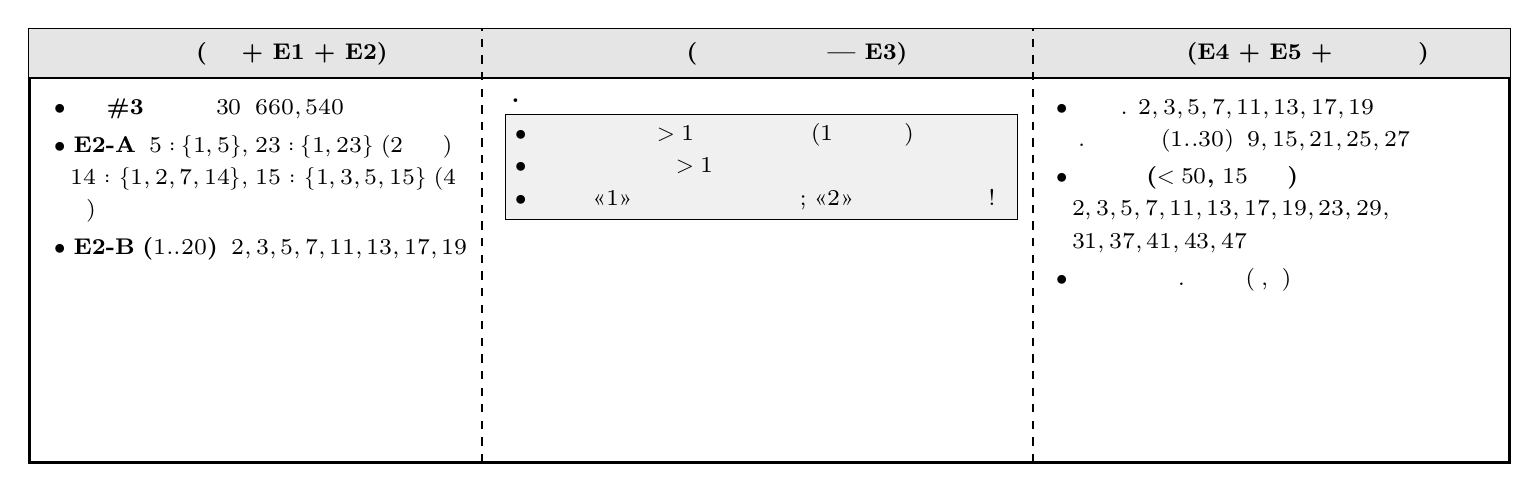
\begin{tikzpicture}[x=1cm, y=1cm, every node/.style={font=\fontsize{8.2pt}{11.6pt}\selectfont, text=black}]
  \draw[black, line width=1.1pt] (0,0) rectangle (18.8,5.50);
  \fill[gray!20] (0,4.88) rectangle (18.8,5.50);
  \draw[black, line width=0.7pt] (0,4.88) -- (18.8,4.88);
  \draw[black, dashed, line width=0.7pt] (5.75,0) -- (5.75,5.50);
  \draw[black, dashed, line width=0.7pt] (12.75,0) -- (12.75,5.50);

  \node at (2.875,5.19) {\textbf{ផ្នែកឆ្វេង (កំណែ + \en{E1} + \en{E2})}};
  \node at (9.25,5.19) {\textbf{ផ្នែកកណ្ដាល (ខ្លឹមសារគោលរក្សាទុក — \en{E3})}};
  \node at (15.775,5.19) {\textbf{ផ្នែកស្ដាំ (\en{E4} + \en{E5} + កិច្ចការផ្ទះ)}};

  % Left
  \node[anchor=north west, text width=5.30cm] at (0.20,4.74) {%
    $\bullet$ \textbf{កំណែ \#3៖} ពហុគុណនៃ $30$៖ $660, 540$\\[2pt]
    $\bullet$ \textbf{\en{E2-A}៖} $5:\{1,5\}$, $23:\{1,23\}$ ($2$ តួចែក)\\
    \hspace*{0.2cm}$14:\{1,2,7,14\}$, $15:\{1,3,5,15\}$ ($4$ តួចែក)\\[2pt]
    $\bullet$ \textbf{\en{E2-B} ($1..20$)៖} $2,3,5,7,11,13,17,19$
  };

  % Center
  \node[anchor=north west, text width=6.65cm] at (5.92,4.74) {%
    {\muol\fontsize{8.3pt}{11.8pt}\selectfont ៣\enbf{.} ចំនួនបឋម និងចំនួនមិនបឋម}\\[3pt]
    \tikz\node[draw=black, fill=gray!12, inner sep=3.5pt, text width=6.25cm]{%
      $\bullet$ \textbf{ចំនួនបឋម៖} ចំនួនគត់ $>1$ មានតួចែក\textbf{តែពីរគត់} ($1$ និងខ្លួនឯង)\\
      $\bullet$ \textbf{ចំនួនមិនបឋម៖} ចំនួនគត់ $>1$ មានតួចែក\textbf{ច្រើនជាងពីរ}\\
      $\bullet$ \textbf{សម្គាល់៖} «$1$» មិនមែនបឋម និងមិនមែនមិនបឋម; «$2$» ជាចំនួនបឋមគូតែមួយគត់!
    };
  };

  % Right
  \node[anchor=north west, text width=5.65cm] at (12.92,4.74) {%
    $\bullet$ \textbf{គំរូ៖} ក. $2,3,5,7,11,13,17,19$\\
    \hspace*{0.2cm}ខ. មិនបឋមសេស ($1..30$)៖ $9,15,21,25,27$\\[2pt]
    $\bullet$ \textbf{ប្រតិបត្តិ ($<50$, $15$ ចំនួន)៖}\\
    \hspace*{0.2cm}$2,3,5,7,11,13,17,19,23,29,$\\
    \hspace*{0.2cm}$31,37,41,43,47$\\[2pt]
    $\bullet$ \textbf{កិច្ចការផ្ទះ៖} ទំ.២៤ លេខ ៤ (ក, ខ)
  };
\end{tikzpicture}
\end{center}

\vfill
\secstrip{២. ចម្លើយផ្ទៀងផ្ទាត់រហ័សសម្រាប់សន្លឹកកិច្ចការសិស្ស \enbf{(}ទំព័រ ១ និង ទំព័រ ២\enbf{)}}{\en{Answer Key}}

\begin{tcolorbox}[
  enhanced, sharp corners, colback=white, colframe=black,
  boxrule=0.8pt, boxsep=2.5pt, top=4pt, bottom=4pt, left=6pt, right=6pt
]
  \fontsize{8.8pt}{13.0pt}\selectfont
  $\bullet$ \textbf{ផ្នែក \en{E1}៖} \textbf{សិស្ស ខ} ត្រឹមត្រូវ ។ \textbf{ផ្នែក \en{E2-A}៖} $14$ ($1,2,7,14 \to 4$ តួចែក, ចំនួនមិនបឋម); $15$ ($1,3,5,15 \to 4$ តួចែក, ចំនួនមិនបឋម); $23$ ($1,23 \to 2$ តួចែក, ចំនួនបឋម); $2$ ($1,2 \to 2$ តួចែក, ចំនួនបឋម); $1$ ($1$ តួចែកគត់) ។\\[2pt]
  $\bullet$ \textbf{ផ្នែក \en{E4}៖} ក. $\mathbf{2, 3, 5, 7, 11, 13, 17, 19}$; ខ. $\mathbf{9, 15, 21, 25, 27}$ ។ \en{EIA}៖ $11\times 11 = \mathbf{121} > 50$ ។\\[2pt]
  $\bullet$ \textbf{ផ្នែក \en{E5}៖} ១) ចំនួនបឋមតូចជាង $50$ មាន $\mathbf{15}$ ចំនួនគឺ $\mathbf{2, 3, 5, 7, 11, 13, 17, 19, 23, 29, 31, 37, 41, 43, 47}$ ។ ៣) \textbf{ជម្រើស \en{C}} ។ ៤) សំបុត្រចេញ៖ បឋមគឺ $\mathbf{2, 29}$; មិនបឋមគឺ $\mathbf{21, 49}$ ។
\end{tcolorbox}

\vfill
\secstrip{៣. ចម្លើយលម្អិតនៃកិច្ចការផ្ទះ \enbf{(}សៀវភៅគោល ទំ.២៤ លេខ ៤\enbf{)}}{សៀវភៅគោល ទំ.២៤}

\begin{tcolorbox}[
  enhanced, sharp corners, colback=white, colframe=black,
  boxrule=0.8pt, boxsep=2.5pt, top=4pt, bottom=4pt, left=6pt, right=6pt
]
  \fontsize{8.7pt}{12.8pt}\selectfont
  $\bullet$ \textbf{លេខ ៤ ក. (តួចែកនៃចំនួននីមួយៗ)៖} $11:\{1,11\}$; \ $15:\{1,3,5,15\}$; \ $17:\{1,17\}$; \ $18:\{1,2,3,6,9,18\}$; \ $19:\{1,19\}$; \ $20:\{1,2,4,5,10,20\}$; \ $21:\{1,3,7,21\}$; \ $22:\{1,2,11,22\}$; \ $23:\{1,23\}$; \ $29:\{1,29\}$ ។\\[2pt]
  $\bullet$ \textbf{លេខ ៤ ខ. (ចំនួនបឋម)៖} គឺចំនួនដែលមានតួចែកតែពីរគត់៖ $\mathbf{11,\ 17,\ 19,\ 23,\ 29}$ ($5$ ចំនួន) ។
\end{tcolorbox}

\vfill
\secstrip{៤. ចំណុចប្រុងប្រយ័ត្នគរុកោសល្យសម្រាប់គ្រូ \enbf{(}អន្ទាក់ចំនួនបឋមក្លែងក្លាយ\enbf{)}}{\en{Pedagogical Watchlist}}

\begin{tcolorbox}[
  enhanced, sharp corners, colback=panelgray, colframe=black,
  boxrule=0.85pt, boxsep=2.5pt, top=4pt, bottom=4pt, left=6pt, right=6pt
]
  \fontsize{8.6pt}{12.6pt}\selectfont
  $\bullet$ \textbf{ចំនួនសេសដែលសិស្សឧស្សាហ៍ច្រឡំថាបឋម៖} $9=3^2$, $15=3\times 5$, $21=3\times 7$, $25=5^2$, $27=3^3$, $33=3\times 11$, $39=3\times 13$, $\mathbf{49=7\times 7}$, $\mathbf{51=3\times 17}$ ($5+1=6\div 3$!), $\mathbf{57=3\times 19}$ និង $\mathbf{91=7\times 13}$ ។\\[2pt]
  $\bullet$ \textbf{សំណួរចងចាំរហ័ស៖} «តើមានចំនួនបឋមគូប៉ុន្មានចំនួន?» $\to$ មានតែ $1$ គត់គឺលេខ $\mathbf{2}$! រាល់ចំនួនគូធំជាង $2$ សុទ្ធតែចែកដាច់នឹង $2$ (មិនបឋម) ។
\end{tcolorbox}

\end{document}
